%% plainproblemname: Fotografen
\problemname{Fotografen}
En fotograf har tagit många fina foton med sin digitalkamera och kopplar in den
i sin dator för att överföra bilderna. Bilderna har tagits med olika vridningar
av kameran så nu är vissa av bilderna roterade. Vi kallar de fyra möjliga
rotationerna ett foto kan ha för \emph{upp}, \emph{höger}, \emph{ner} och \emph{vänster} och
definierar det som den sida som motsvarar uppåt i bilden. En bild är vänd rätt
om den är roterad \emph{upp}. Datorn visar bilderna i en lista och har en funktion
som roterar en bild $90^\circ$ medurs. Rotationen sker alltså enligt följande ordning:

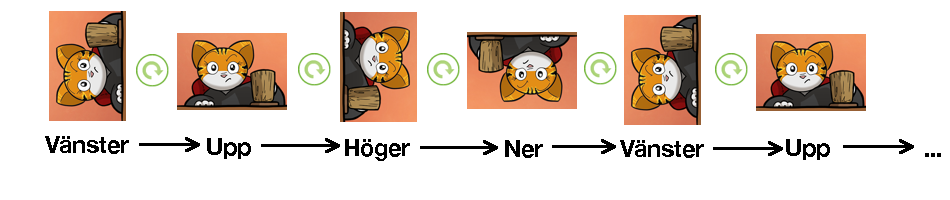
\includegraphics[width=0.8\textwidth]{fotografen.png}

Fotografen tycker det verkar tråkigt att rotera foton och bestämmer sig för att
göra det till ett roligt spel. Fotografen väljer ett positivt heltal $k$ och
bestämmer att det enda sättet att rotera foton är att rotera $k$ på varandra
följande foton samtidigt. Listan med foton har en början och ett slut, den är
inte cyklisk. Formellt har fotografen $N$ foton, kalla dem $a_1, a_2, \dots
a_N$. Fotografen kan nu välja ett index $i$ ($1 \leq i \leq N-k+1$)
och bilderna $a_i, a_{i+1}, ... , a_{i+k-1}$ roteras då $90^\circ$ medurs. Detta kallar vi en
operation.

Målet med spelet är att vända alla foton rätt med så få operationer som
möjligt. Skriv ett program som beräknar det minsta antalet operationer som krävs.

\section*{Indata}
På första raden står två heltal $N$ och $k$ ($1 \leq k \leq N \leq 100\,000$),
antalet foton totalt respektive antalet foton som måste roteras samtidigt.
På andra raden står $N$ tecken som representerar fotografiernas rotation från
början: \texttt{U} för upp, \texttt{H} för höger, \texttt{N} för ner och
\texttt{V} för vänster.

\section*{Utdata}
Skriv ut det minsta antalet operationer som krävs. Om det inte går att vända
alla foton rätt, skriv ut $-1$.

\section*{Exempel}
För det första exempelindatat så är en möjlig optimal lösning denna: Rotera
tre gånger på position 3-4 för att få \texttt{UVVU}, rotera sedan en gång på
position 2-3 för att slutligen få \texttt{UUUU}, och vi är klara med fyra
operationer utförda.

\section*{Delpoäng} I det här problemet kan du samla en del av poängen utan att
lösa problemet fullständigt.

\begin{itemize}
    \item För 10 poäng så kommer $N$ vara maximalt 10.
    \item För ytterligare 40 poäng så kommer $N$ vara maximalt $5\,000$.
\end{itemize}
